\documentclass[a4paper,11pt]{book}

% Sprach- und Zeichencodierung
\usepackage[T1]{fontenc}       % korrekte Darstellung von Umlauten
\usepackage[utf8]{inputenc}    % UTF-8 Eingabekodierung
\usepackage[german]{babel}    % deutsche Spracheinstellungen
\usepackage{microtype}

% Mathematik
\usepackage{amsmath, amssymb, mathtools} % erweiterte Matheumgebungen
\usepackage{siunitx}                     % SI-Einheiten und Zahlenformatierung
\sisetup{per-mode=symbol}

% Layout und Formatierung
\usepackage{geometry}          % Seitenränder einstellen
\usepackage{graphicx}          % Grafiken einbinden
\usepackage{pdfpages}


\usepackage{float}             % präzise Positionierung von Bildern
\usepackage{fancyhdr}          % Kopf- und Fußzeilen
\usepackage{titlesec}          % Überschriftenformatierung
\usepackage{tocloft}           % Inhaltsverzeichnis anpassen
\usepackage{makecell}          % Zeilenumbrüche in Tabellenzellen
\usepackage{array}             % erweiterte Tabellenspalten
\usepackage{booktabs,tabularx} % schöne Tabellen
\usepackage{longtable}         % Tabellen über mehrere Seiten
\usepackage{caption}           % bessere Bild-/Tabellenunterschriften
\usepackage{subcaption}        % Subfigures
\usepackage{enumitem}          % flexible Listen
\usepackage{subfiles}           % Kapitel einzeln kompilierbar
\usepackage{tikz}
\usepackage{circuitikz}
\usetikzlibrary{arrows.meta, positioning}

\usepackage{pgfplots}
\pgfplotsset{compat=1.18}
%\newcommand{\datapath}{../../003_Messdaten}
\usepgfplotslibrary{groupplots}

% Literatur
\usepackage{csquotes}                           % saubere Anführungszeichen
\usepackage[backend=biber, style=ieee]{biblatex} % IEEE-Stil mit Biber
\addbibresource{Literaturverzeichnis.bib}       % Literaturdatenbank einbinden
\usepackage[acronym]{glossaries-extra}
\setabbreviationstyle[acronym]{long-short}
\newacronym{pll}{PLL}{Phase-Locked Loop}%

%\newacronym{digipot}{DP}{Digitalpotentiometer}

\newacronym{opv}{OPV}{Operationsverstärker}%fertig

\newacronym{pd}{PD}{Phasendetektor}%

\newacronym{vco}{VCO}{Voltage-Controlled Oscillator}%

\newacronym{vcf}{VCF}{Voltage-Controlled Filter}%

\newacronym{pcb}{PCB}{Printed Circuit Board}%

\newacronym{mcu}{MCU}{Microcontroller Unit}%

\newacronym{gpio}{GPIO}{General Purpose Input Output}

\newacronym{spi}{SPI}{Serial Peripheral Interface}

\newacronym{adc}{ADC}{Analog Digital Converter}%

\newacronym{ui}{UI}{User Interface}

\newacronym{wlan}{WLAN}{Wireless Local Area Network}

\newacronym{eeprom}{EEPROM}{Electrically Erasable Programmable Read-Only Memory}

\newacronym{http}{HTTP}{Hypertext Transfer Protocol}

\newacronym{html}{HTML}{Hypertext Markup Language}

\newacronym{ip}{IP}{Internet Protocol}

\newacronym{ram}{RAM}{Random Access Memory}

\newacronym{gbw}{GBW}{Gain Bandwidth Product}

%\newacronym{sf}{SF}{Scale Factor}

\newacronym{ic}{IC}{Integrated Circuit}

\newacronym{dut}{DUT}{Device Under Test}
\makeglossaries

% Zusatzfunktionen
\usepackage{lastpage}    % für "Seite X von Y"
\usepackage{xcolor}      % Farben (für Listings etc.)
\usepackage{listings}    % Codeblöcke
\usepackage[hidelinks]{hyperref} % Hyperlinks (immer zuletzt)


% Einstellungen für Code
\lstset{
    basicstyle=\ttfamily\scriptsize, % Sehr kleine Schrift für Platzersparnis
    breaklines=true,                 % Automatische Zeilenumbrüche
    frame=tb,                        % Linien oben und unten
    tabsize=2,
    literate={Ω}{{\textOmega}}1,     % Ersetzt das Omega-Zeichen durch LaTeX-Befehl
    extendedchars=true,
    inputencoding=utf8
}


% Seitenlayout
\geometry{
  top=2cm,
  bottom=3cm,
  left=2.5cm,
  right=2.5cm
}
\setlength\parindent{0pt} % kein Absatzeinzug


% Kopf- und Fußzeilen
\setlength\headheight{55pt}%26
\setlength\headsep{15pt}%35
\addtolength{\topmargin}{-12pt}

\pagestyle{fancy}
\fancyhf{}
\lhead{\raisebox{-0.2cm}{\includegraphics[height=1cm]{Bilder/hsb_logo2.png}}}
\chead{Bachelor Thesis\par Nils Renner}
\rhead{\raisebox{-0.2cm}{\includegraphics[height=1.3cm]{Bilder/hsb_logo1.png}}}
\cfoot{\thepage}


% Dokumentbeginn
\begin{document}

\frontmatter
\pagenumbering{roman}
\pagestyle{empty} % unterdrückung des headers
\setcounter{page}{1}

% Titelseite
\begin{titlepage}
    \begin{center}
    \includegraphics[width=0.6\textwidth]{Bilder/Logo_HSB_Hochschule_Bremen.png}\\[1cm]
    \vspace{0.5cm}
    {\huge\bfseries Implementierung eines selbsteinstellenden Filters auf Basis eines spannungsgesteuerten Biquad-Filters\par}
    \vspace{1.5cm}
    {\large\bfseries Implementation of a Self-Tuned Filter Based on a Voltage-Controlled Biquad Filter\par}
    
    \vspace{2cm}
    {\Large\bfseries Bachelor Thesis\par}
    {\large Fakultät 4: Elektrotechnik und Informatik\par} 
    {\large Studiengang: Elektrotechnik B. Eng.\par}
    {\large Vertiefungsrichtung: Informationstechnik\par}
    %Presented for Attainment of the Academic Degree of \par
    %Bachelor of Engineering at the City University of Applied Sciences Bremen\par
    \end{center}
    \vspace{2cm}

    \begin{tabular}{l l}
            \textbf{Autor:} & Nils Renner, Wulfhoopstraße 34a, 28201 Bremen \\
            \textbf{Matr.-Nr.:} & 5197659 \\
            \textbf{Abgabetermin:} & 2. März, 2026 \\ \\ \\
            \textbf{Prüfer:} & Prof. Dr.-Ing. Mirco Meiners,\\ & \small{Hochschule Bremen,}\\ & \small{Concept Engineering SoCs and Design}\\ \\
            \textbf{} & Prof. Dr. Sören Peik,\\ & \small{Hochschule Bremen,}\\ & \small{Microwave Technology and Satellite Communications} \\
    \end{tabular}

    \vfill
\end{titlepage}

\newpage
\null
\thispagestyle{empty} 


% Erklärung zur selbstständigen Arbeit
\clearpage{\pagestyle{empty}\cleardoublepage}
%\cleardoublepage % Sorgt dafür, dass das Kapitel auf einer neuen (rechten) Seite beginnt
\phantomsection 
\addcontentsline{toc}{chapter}{Erklärung über das Eigenständige Erstellen der Arbeit} 

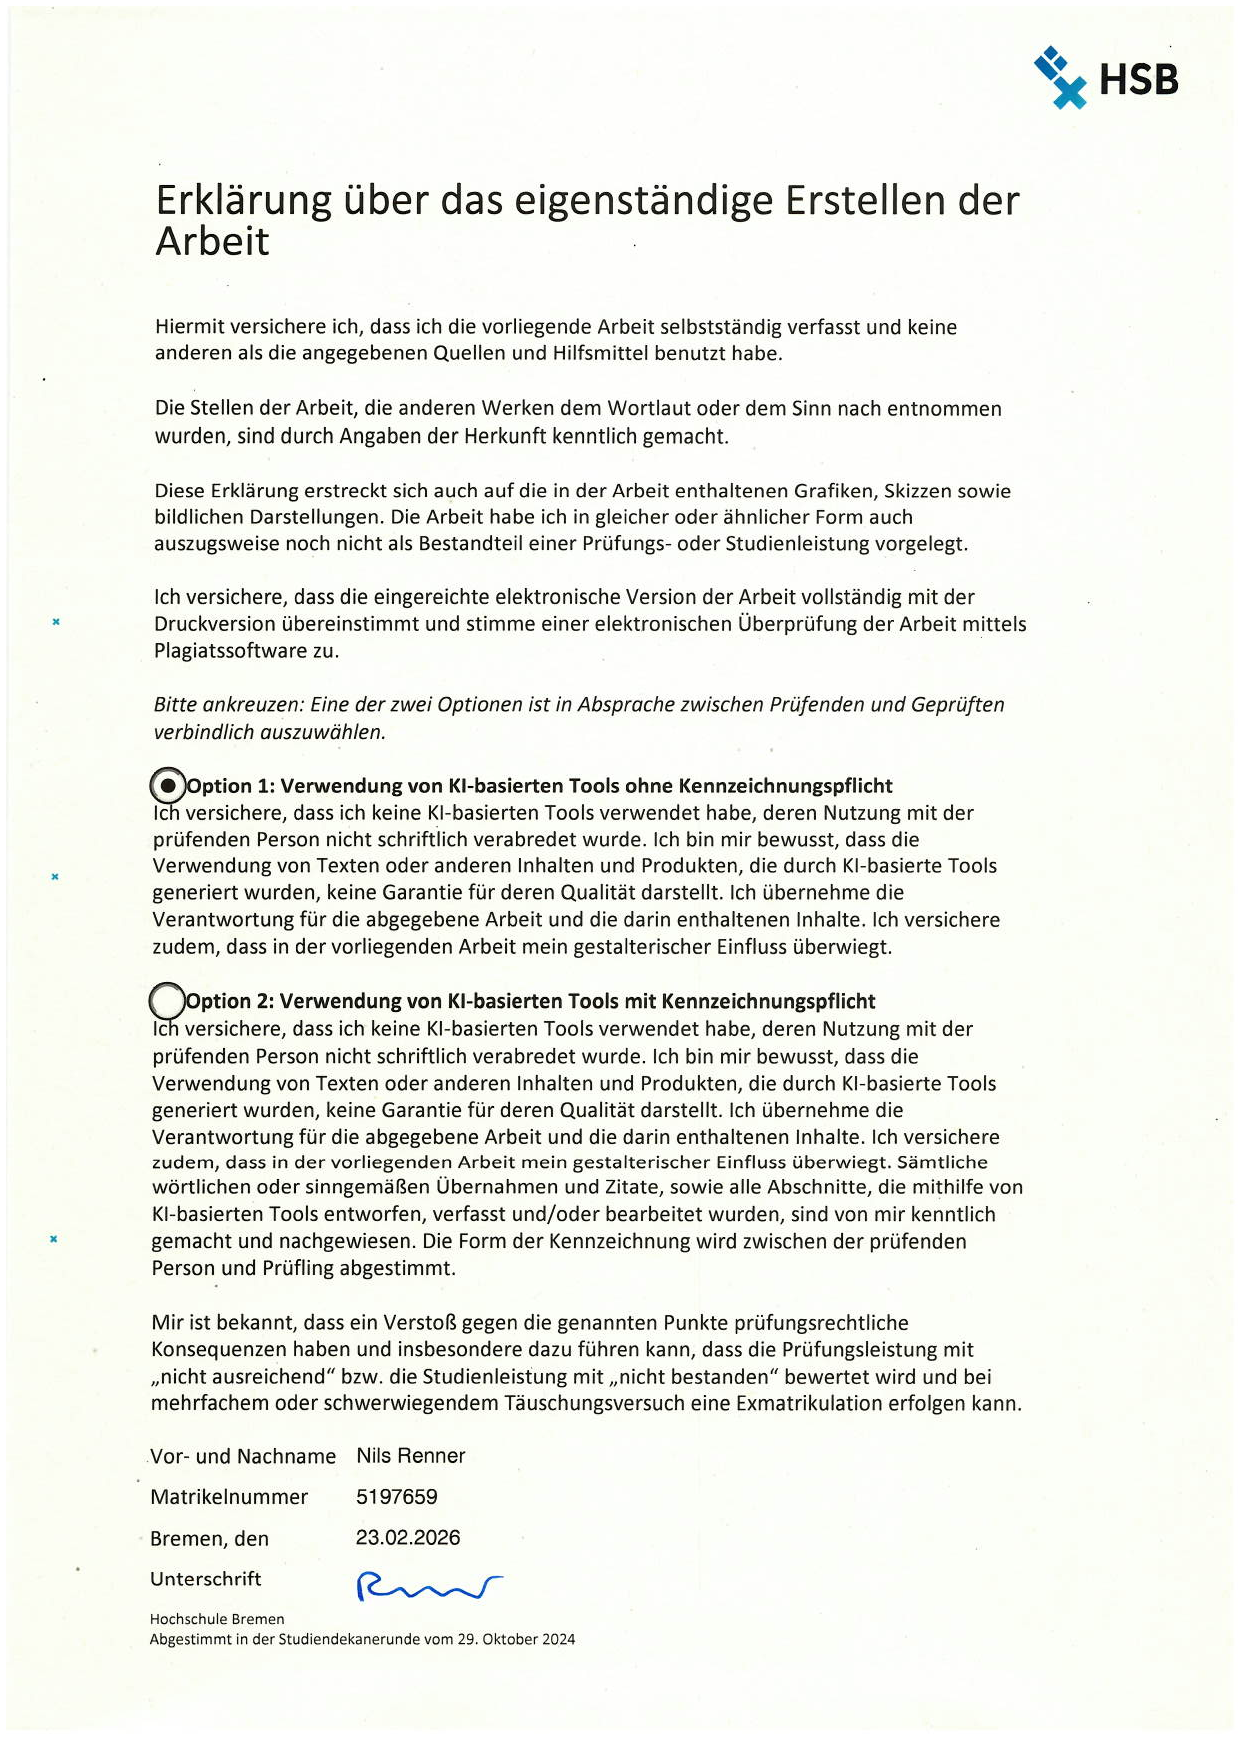
\includepdf[pages={1}, scale=1, pagecommand={}]{KI-Eigenständigkeitserklärung_Renner.pdf}








% Acknowledgements / Danksagung
\clearpage{\pagestyle{empty}\cleardoublepage}
\chapter*{Danksagung}
\addcontentsline{toc}{chapter}{Danksagung}

An dieser Stelle möchte ich mich bei all jenen bedanken, die mich während der Erstellung dieser Bachelorarbeit unterstützt haben.\par
\medskip
Mein besonderer Dank gilt Herrn Prof. Dr.-Ing. Mirco Meiners für die Übernahme der Erstbetreuung sowie für die wertvollen Anregungen und konstruktiven Vorschläge während der Bearbeitungszeit.\par
\medskip
Ebenso bedanke ich mich herzlich bei Herrn Dipl.-Ing. Tim Ziemann für das Layout-Review und die damit verbundene Beratung.\par
\medskip
Für die technische Unterstützung danke ich Simon Cossens, der mir bei allen Fragen rund um die hardwaretechnischen Anforderungen stets als kompetenter Ansprechpartner zur Seite stand.\par
\medskip
Ein großes Dankeschön für das gründliche Korrekturlesen und das hilfreiche Feedback gebührt zudem Ali Mert Ackey, Alicia von Ahlen, Daniel Albinger, Janik Holland, Melia Keil, Finn Ringelsiep, Julian Scheeler und Jana Vogt.\par
\medskip
Abschließend möchte ich mich noch bei meinem Vater für den kontinuierlichen Austausch über meine Ideen und Pläne sowie für die wertvolle kritische Reflexion während des gesamten Prozesses bedanken. 



% Abstract
\clearpage{\pagestyle{empty}\cleardoublepage}
\chapter*{Abstrakt}
\addcontentsline{toc}{chapter}{Abstrakt}
Die vorliegende Bachelorarbeit befasst sich mit dem Design, der Simulation und der messtechnischen Verifizierung eines analogen, selbsteinstellenden Filters (Self-Tuned Filter). Ziel der Arbeit war die Entwicklung eines Systems, das seine Resonanzfrequenz eigenständig an die anliegende Eingangsfrequenz anpasst. \par
\medskip

Im Rahmen der Arbeit wurde ein PCB entwickelt, auf dem ein Raspberry Pi Pico 2 W als zentrale Steuereinheit und digitale Schnittstelle dient. Über eine webbasierte Benutzeroberfläche können die Filterparameter über Digitalpotentiometer gesteuert und die mithilfe des Nulldurchgangszählers ermittelte Frequenz systematisch erfasst und visualisiert werden. Ein wesentlicher Teil der Arbeit bestand in der eigenständigen Herleitung und Verifikation der Gleichungen zur Resonanzfrequenz des Systems, wodurch ein umfassendes Verständnis der physikalischen Zusammenhänge innerhalb des Self-Tuned Filters aufgebaut werden konnte.\par
\medskip

Ein zentrales Ergebnis der Arbeit ist der Nachweis der Funktionalität des Systems in einem Frequenzbereich von ca. \SI{240}{\hertz} bis über \SI{12}{\kilo\hertz}. Dabei konnte gezeigt werden, dass die Stabilität der Regelung maßgeblich von der Amplitude des Eingangssignals abhängt. Durch eine gezielte Pegelanpassung auf \SI{0.5}{\volt} wurde der störende AC-Anteil auf der Steuerspannung um über \SI{80}{\percent} reduziert, was den operativen Arbeitsbereich des Filters signifikant erweiterte. Die Arbeit belegt somit die erfolgreiche Realisierung eines stabilen, selbsteinstellenden Filtersystems.\par
\medskip

\section*{Abstract}
This bachelor thesis deals with the design, simulation, and metrological verification of an analog, self-tuning filter. The aim of the thesis was to develop a system that independently adjusts its resonance frequency to the applied input frequency. \par
\medskip

As part of the thesis, a PCB was developed on which a Raspberry Pi Pico 2 W serves as the central control unit and digital interface. Via a web-based user interface, the filter parameters can be controlled via digital potentiometers and the frequency determined using the zero-crossing counter can be systematically recorded and visualized. A significant part of the work consisted of independently deriving and verifying the equations for the resonance frequency of the system, which enabled a comprehensive understanding of the physical relationships within the self-tuned filter to be established.\par
\medskip

A key result of the work is the verification of the system's functionality in a frequency range from approximately \SI{240}{\hertz} to over \SI{12}{\kilo\hertz}. It was shown that the stability of the control depends significantly on the amplitude of the input signal. By specifically adjusting the level to \SI{0.5}{\volt}, the disruptive AC component on the control voltage was reduced by over \SI{80}{\percent}, which significantly expanded the filter's operational range. The work thus demonstrates the successful implementation of a stable, self-adjusting filter system.\par
\medskip





% Inhaltsverzeichnis
\clearpage{\pagestyle{empty}\cleardoublepage}
\tableofcontents


% Abbildungsverzeichnis
\clearpage{\pagestyle{empty}\cleardoublepage}
\listoffigures
\addcontentsline{toc}{chapter}{Abbildungsverzeichnis}



% Tabellenverzeichnis 
\clearpage{\pagestyle{empty}\cleardoublepage}
\listoftables
\addcontentsline{toc}{chapter}{Tabellenverzeichnis}



% Abkürzungsverzeichnis
\clearpage{\pagestyle{empty}\cleardoublepage}
\printglossary[type=\acronymtype, title=Abkürzungsverzeichnis, nonumberlist]
%\addcontentsline{toc}{chapter}{Abkürzungsverzeichnis}



\mainmatter
\pagestyle{fancy}
% Haupttext
% \newpage  
\pagenumbering{arabic}  
\setcounter{page}{1}

\subfile{Einleitung/Einleitung.tex}

% \newpage
\subfile{Tools/Tools.tex}

% \newpage
\subfile{Theorie/Theorie_alt.tex}
% \newpage
\subfile{Theorie/Theorie_neu.tex}

% \newpage
\subfile{Simulation/Simulation.tex}

% \newpage
\subfile{systemdesign/systemdesign.tex}

% \newpage
\subfile{Messung/Messung.tex}

% \newpage
\subfile{Auswertung/Auswertung.tex}

% \newpage
\subfile{Fazit/Fazit.tex}

\backmatter
\appendix
% \newpage
\printbibliography



\newpage
\chapter{Messmittel}
\begin{table}[h]
    \centering
    \begin{tabular}{c|c|c|c}
        \textbf{Messmittel} & \textbf{Hersteller} & \textbf{Bezeichnung} & \textbf{Gerätenummer} \\ \hline
        Oszilloskop & Rohde \& Schwarz & RTB2002 & 75669148 \\
        Signalgenerator & RIGOL & DG1032 & 75001816 \\
        Red Pitaya & Red Pitaya & STEMlab 125-14 & - \\
        Multimeter & Fluke & 175 & 1600 5357 \\
    \end{tabular}
\end{table}





\newpage
\chapter{KI-Prompt-Engineering}

\section{Erstellung einer python Simulation eines Slef-Tuned Filters anhand einer diskreten und proportionalen Regelung}

Für diesen Prompt wurde Le Chat von Mistral verwendet. \par
\medskip

\begin{enumerate}
\item \textbf{Rolle:} Experte für Python-Programmierung und Signalverarbeitung.
\item \textbf{Ziel:} Erstelle eine Python-Simulation eines Self-Tuned Filters (VCF), die exakt das Verhalten einer diskreten Stufenregelung auf Basis der Phasenlage abbildet.
\item \textbf{Logik:} Erzeuge ein Referenz-Sinussignal (\SI{1000}{\hertz}) und ein VCF-Signal (Start: \SI{1050}{\hertz}). Prüfe die Phase des VCF-Signals exakt an den positiven Nulldurchgängen der Referenz.
\item \textbf{Regelgesetz:} Befindet sich die Phase im Bereich von \SI{-90}{\degree} bis \SI{90}{\degree}, wird die Frequenz um \SI{10}{\hertz} erhöht; andernfalls wird sie um \SI{10}{\hertz} verringert.
\item \textbf{Implementierung:} Das VCF-Signal muss durch fortlaufende Integration der Phase berechnet werden , um Phasensprünge bei Frequenzänderungen zu vermeiden.
\end{enumerate}

Anschließend wird der Code erweitert, sodass die Frequenzsprünge proportional anhand der Phasenlage verändert werden.\par
\medskip

\begin{enumerate}
\item \textbf{Ziel:} Modifiziere die vorherige Simulation hin zu einer proportionalen Regelung (P-Regler).
\item \textbf{Setup:} Erhöhe die Simulationsdauer auf \SI{0.5}{\second}.
\item \textbf{Logik:} Die Frequenzänderung soll nun kontinuierlich erfolgen. Die Stärke der Korrektur  wird über eine trigonometrische Gewichtung (z. B. Absolutwert des Cosinus der Phase) gesteuert.
\item \textbf{Verhalten:} Dies stellt sicher, dass in der Umgebung von \SI{0}{\degree} und \SI{180}{\degree} maximale Frequenzänderungen resultieren, während die Korrektur an den Arbeitspunkten \SI{90}{\degree} und \SI{270}{\degree} gegen Null strebt.
\item \textbf{Richtung:} Ist die Phase im Bereich von \SI{-90}{\degree} bis \SI{90}{\degree} soll die Frequenz erhöht werden, andernfalls wird die Frequenz verringert.
\end{enumerate}


\newpage

\section{Erstellung des HTTP-Server und Erweiterung des Frequenzzählers}
\label{sec:prompt3}

Dieser Prompt dient der finalen Migration des Projekts auf Hardware-gestützte Frequenzmessung. Für diesen Prompt wurde Gemini 3 Flash von Google verwendet. \par
\medskip

\begin{enumerate}
    \item \textbf{Rolle:} Experte für Embedded Systems (RP2350) und Python-Webentwicklung.
    \item \textbf{Ziel:} Erweitere mein Python-Skript für einen Raspberry Pi Pico (RP2040). Der aktuelle Code enthält eine SPI-Ansteuerung für Digitalpotentiometer, einen Webserver im AP-Modus und einen IRQ-Frequenzzähler.
    \item \textbf{Upgrade:} Ersetze den IRQ-Zähler durch einen PIO-Zähler (Pin 21). Die CPU darf nicht blockiert werden. Implementiere einen \texttt{machine.Timer} (2s Intervall), der den Wert ausliest und auf 1 Hz rundet. Speichere die letzten 5 Messwerte.
    \item \textbf{UI:} Erstelle ein zweispaltiges HTML-Layout. Links: Eingabefelder für Frequenz, Güte und Verstärkung sowie aktuelle Zustände. Rechts: Tabelle der letzten 5 Messwerte. Auto-Refresh: 15s.
    \item \textbf{Performance:} Der Webserver muss sofort reagieren (Nutzung globaler Variablen).
    \item \textbf{Basis-Code:}
\end{enumerate}

\lstset{
    basicstyle=\ttfamily\scriptsize,
    breaklines=true,
    extendedchars=true,
    literate={-}{{-}}1 % Verhindert Probleme mit Bindestrichen
}

\begin{lstlisting}[caption={Basis-Code Teil 1: Setup und Logik}]
import math
from machine import Pin, SPI
import network, socket, time

led = Pin("LED", Pin.OUT)
for _ in range(5):
    led.value(1); time.sleep(0.1)
    led.value(0); time.sleep(0.1)
led.value(1)

# Parameter und Berechnungen
freq0, Q_val, H0_val = 160, 1, 1
max_step, r_ges, wiper_r = 255, 9650, 4

def clamp_and_round(x):
    return int(round(max(0, min(255, x))))

def freq_2_bit(f0):
    w0 = f0 * 2 * 3.14159
    r = 1/(w0 * 1e-6)
    wiper = max_step * (1 - r/r_ges) + wiper_r
    return clamp_and_round(wiper), r

def Q_2_bit(Q_val):
    r_opv = 1000
    Q_r = Q_val * r_opv
    Q_wiper = max_step * (1 - Q_r/r_ges) + wiper_r
    return clamp_and_round(Q_wiper), Q_r

def H0_2_bit(H0_val):
    r_opv = 1000
    H0_r = r_opv/H0_val
    H0_wiper = max_step * (1 - H0_r/r_ges) + wiper_r
    #H0_wiper = int(round(H0_wiper))
    return clamp_and_round(H0_wiper), H0_r

def bit_2_res(bit):
    res = r_ges * (1 - (bit-wiper_r)/max_step) 
    return res

\end{lstlisting}

\begin{lstlisting}[caption={Basis-Code Teil 2: Hardware-Schnittstellen}]
def update_filter(f, q, h):
    fw, fr = freq_2_bit(f)
    set_wiper0(cs1, fw); set_wiper1(cs1, fw)

# Hardware Konfiguration (SPI & Pins)
spi = SPI(0, baudrate=1000000, sck=Pin(18), mosi=Pin(19), miso=Pin(16))
cs1, cs2 = Pin(17, Pin.OUT, value=1), Pin(20, Pin.OUT, value=1)

def mcp_write(cs, cmd, val):
    cs.value(0)
    spi.write(bytes([cmd & 0xFF, val & 0xFF]))
    cs.value(1)

def set_wiper0(c, v): mcp_write(c, 0, v)
def set_wiper1(c, v): mcp_write(c, 16, v)

# WLAN Access Point starten
ap = network.WLAN(network.AP_IF)
ap.active(True)
ap.config(essid="Pico-Filter", password="filter123")
ap.ifconfig(("192.168.4.1", "255.255.255.0", "192.168.4.1", "8.8.8.8"))
\end{lstlisting}







\end{document}
